\documentclass[tikz,border=5pt]{standalone}

\begin{document}
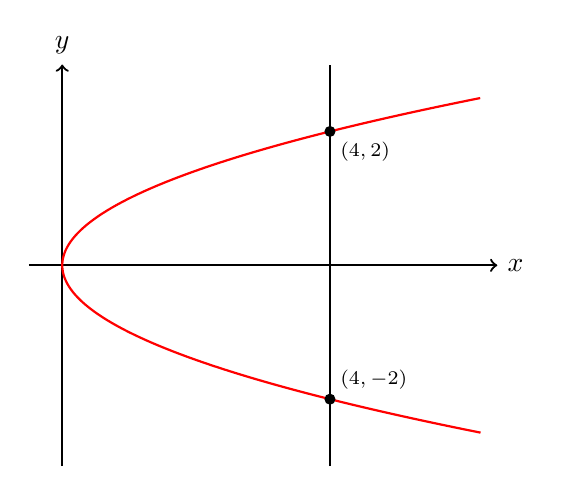
\begin{tikzpicture}[x=0.85cm,y=0.85cm, thick]

  % Axes
  \draw[->] (-0.5,0) -- (6.5,0) node[right] {$x$};
  \draw[->] (0,-3) -- (0,3) node[above] {$y$};

  % Graph of x = y^2 (red)
  \draw[red, thick, variable=\t, domain=-2.5:2.5, samples=120]
    plot ({\t*\t}, {\t});

  % Vertical line x = 4 (black)
  \draw[black] (4,-3) -- (4,3);

  % Intersection points (black)
  \fill[black] (4,2)  circle (2pt);
  \fill[black] (4,-2) circle (2pt);

  % Optional small labels
  \node[below right, font=\scriptsize] at (4,2)  {$(4,2)$};
  \node[above right, font=\scriptsize] at (4,-2) {$(4,-2)$};

\end{tikzpicture}
\end{document}
